\documentclass[a4paper,10pt,twoside]{article}
\usepackage[polish]{babel}
\usepackage[utf8]{inputenc}
\usepackage[T1]{fontenc}
\usepackage{indentfirst}
\usepackage[top=2.5cm, bottom=2.5cm, left=2.5cm, right=2.5cm]{geometry}
\usepackage{graphicx}
\usepackage{amsmath}
\usepackage{booktabs}

\begin{document}

\newcommand{\unit}[1]{\thinspace \mathrm{#1}}

\begin{center}
\bgroup
\def\arraystretch{1.5}
\begin{tabular}{|c|c|c|c|c|c|}
	\hline
	EAIiIB & \multicolumn{2}{|c|}{Piotr Morawiecki, Tymoteusz Paszun} & Rok II & {Grupa 3a} & {Zespół 6} \\
	\hline
	\multicolumn{3}{|c|}{\begin{tabular}{c}Temat: Moduł Younga \end{tabular}} & 
	\multicolumn{3}{|c|}{\begin{tabular}{c}Numer ćwiczenia: 11 \end{tabular}} \\
	\hline
	\begin{tabular}{@{}c@{}}Data wykonania:\\8.11.2017r.\end{tabular} & \begin{tabular}{@{}c@{}}Data oddania:\\15.11.2017r.\end{tabular} & 
	\begin{tabular}{c}Zwrot do poprawki:\\\phantom{data} \end{tabular} & \begin{tabular}{c}Data oddania:\\\phantom{data}\end{tabular} &
	\begin{tabular}{@{}c@{}}Data zaliczenia:\\\phantom{data}\end{tabular} & \begin{tabular}{c}Ocena:\\\phantom{ocena}\end{tabular} \\[4ex]
	\hline
\end{tabular}
\egroup
\end{center}


\section{Cel ćwiczenia}

Celem ćwiczenia jest wyznaczenie modułu Younga metodą statyczną przy pomocy pomiaru wydłużenia drutu obciążonego stałą siłą. 

\section{Wstęp teoretyczny}


$$ \Delta l = \frac{Fl}{ES} $$

$$ \sigma = E \varepsilon $$

$$ E = \frac{4l}{\pi d^2 a} $$

\section{Opis doświadczenia}

\begin{figure}[!htp]
\centerline{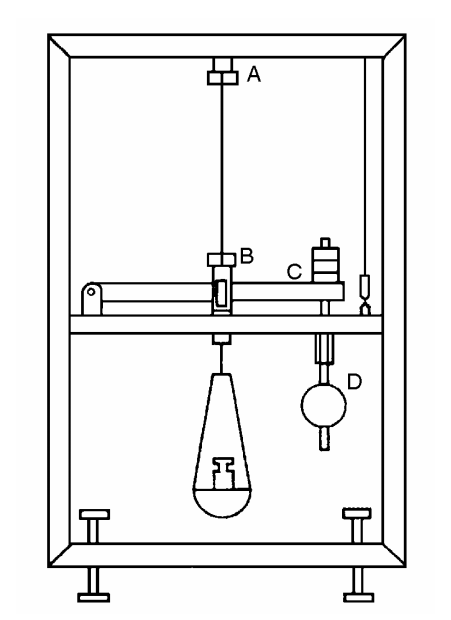
\includegraphics[scale=0.35]{przyrzad.png}}
\caption{Przyrząd pomiarowy}
\label{fig:tl}
\end{figure}

\section{Wyniki pomiarów}

\subsection{Drut stalowy}

Zmierzona długość drutu: $ l = 1065 \unit{mm} $.
Średnica drutu: $ d = \frac{0,715 \unit{mm} + 0,705 \unit{mm} + 0,71 \unit{mm}}{3} = 0,71 \unit{mm}$.

\begin{table}[!htbp]
\caption{Pomiary wydłużenia dla drutu wykonanego ze stali}
\centering
\def\arraystretch{1.4}
\begin{tabular}{@{}rcccc@{}}
\\
\toprule
\begin{tabular}{@{}c@{}}Masa odważników $[\unit{kg}]$\end{tabular} &
\begin{tabular}{@{}c@{}}Siła $F \unit{[N]}$\end{tabular} &
\begin{tabular}{@{}c@{}}Wskazanie czujnika przy \\ dodawaniu obciążenia\end{tabular} &
\begin{tabular}{@{}c@{}}Wskazanie czujnika przy 
\\ odejmowaniu obciążenia\end{tabular} &
\begin{tabular}{@{}c@{}}$\Delta l \unit{[mm]}$\end{tabular}\\
\midrule
0,957  &   9,38817  &  0,290  &  0,38  &  0,16750 \\
1,968  &  19,30608  &  0,780  &  0,83  &  0,40250 \\
2,956  &  28,99836  &  1,110  &  1,17  &  0,57000 \\
3,951  &  38,75931  &  1,425  &  1,48  &  0,72625 \\
4,918  &  48,24558  &  1,780  &  1,78  &  0,89000 \\
5,946  &  58,33026  &  2,070  &  2,07  &  1,03500 \\
6,928  &  67,96368  &  2,320  &  2,38  &  1,17500 \\
7,961  &  78,09741  &  2,630  &  2,65  &  1,32000 \\
8,989  &  88,18209  &  2,915  &  2,92  &  1,45875 \\
9,972  &  97,82532  &  3,230  &        &  1,61500 \\
\bottomrule
\end{tabular}
\end{table}

\subsection{Drut mosiężny}

Zmierzona długość drutu: $ l = 1070,5 \unit{mm} $.
Średnica drutu: $ d = \frac{0,79 \unit{mm} + 0,79 \unit{mm} + 0,795 \unit{mm}}{3} = 0,7917 \unit{mm}$.

\begin{table}[!htbp]
\caption{Pomiary wydłużenia dla drutu wykonanego z mosiądzu}
\centering
\def\arraystretch{1.4}
\begin{tabular}{@{}rcccc@{}}
\\
\toprule
\begin{tabular}{@{}c@{}}Masa odważników $[\unit{kg}]$\end{tabular} &
\begin{tabular}{@{}c@{}}Siła $F \unit{[N]}$\end{tabular} &
\begin{tabular}{@{}c@{}}Wskazanie czujnika przy \\ dodawaniu obciążenia\end{tabular} &
\begin{tabular}{@{}c@{}}Wskazanie czujnika przy 
\\ odejmowaniu obciążenia\end{tabular} &
\begin{tabular}{@{}c@{}}$\Delta l \unit{[mm]}$\end{tabular}\\
\midrule
0,957  &   9,38817  &  0,42  &  0,43  &  0,2125  \\
1,968  &  19,30608  &  0,91  &  0,92  &  0,4575  \\
2,956  &  28,99836  &  1,31  &  1,33  &  0,6600  \\
3,951  &  38,75931  &  1,70  &  1,73  &  0,8575  \\
4,918  &  48,24558  &  2,06  &  2,08  &  1,0350  \\
5,946  &  58,33026  &  2,44  &        &  1,2200  \\
\bottomrule
\end{tabular}
\end{table}

\section{Wykresy}

\begin{figure}[!htp]
\centerline{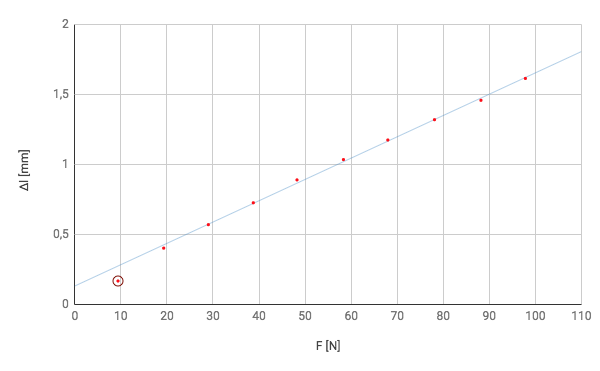
\includegraphics[scale=0.65]{steel_wire_first_point_marked.png}}
\caption{Wykres zależnosci wydłużenia drutu od przyłożonej siły dla stali}
\label{fig:tl}
\end{figure}

\begin{figure}[!htp]
\centerline{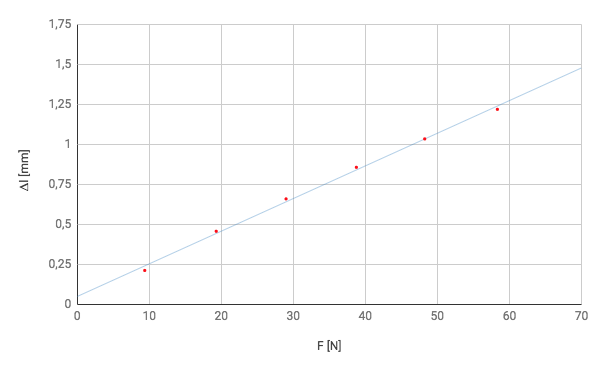
\includegraphics[scale=0.65]{brass_wire.png}}
\caption{Wykres zależnosci wydłużenia drutu od przyłożonej siły dla mosiądzu}
\label{fig:tl}
\end{figure}

\section{Opracowanie wyników}

\subsection{Analiza błędów}

W wynikach pomiarów dla drutu stalowego zauważyliśmy odstawanie pierwszego punktu pomiarowego od prostej wyznaczonej metodą regresji liniowej. W dalszych obliczeniach odrzuciliśmy ten pomiar. Dla drutu wykonanego z mosiądzu nie zauważyliśmy odstawania żadnych punktów pomiarowych.

\subsection{Niepewności pomiarów}

Niepewność pomiaru długości drutu (typu B) - wynika z zastosowania przymiaru o podziałce o dokładności $ 1 \unit{mm} $:

$$ u(l) = \frac{1 \unit{mm}}{\sqrt{3}} = 0,577 \unit{mm} $$

Niepewność pomiaru średnicy drutu (typu B) - wynika z zastosowania śruby mikrometrycznej o dokładności $ 0,01 \unit{mm} $:

$$ u(d) = \frac{0,01 \unit{mm}}{\sqrt{3}} = 0,00577 \unit{mm} $$

Niepewność wpółczynnika kierunkowego $ a = 1,523 \cdot 10^-5 \unit{\frac{m}{N}} $ dla prostej dopasowanej metodą najmniejszych kwadratów dla pomiarów drutu stalowego:

$$ u(a) = 4,275 \cdot 10^8 \unit{\frac{m}{N}} $$

Niepewność wpółczynnika kierunkowego $ a = 2,04 \cdot 10^-5 \unit{\frac{m}{N}} $ dla prostej dopasowanej metodą najmniejszych kwadratów dla pomiarów drutu wykonanego z mosiądzu:

$$ u(a) = 1,36 \cdot 10^7 \unit{\frac{m}{N}} $$

\subsection{Moduł Younga dla drutu stalowego}

Wartość modułu Younga:

$$ E = \frac{4l}{\pi d^2 a} = 176,61 \unit{GPa} $$

Niepewność złożona wyznaczonej wartości modułu Younga:

$$ \frac{u_c(E)}{E} = \sqrt{ \left( \frac{u(l)}{l} \right)^2 + \left( -2 \frac{u(d)}{d} \right)^2 + \left(-\frac{u(a)}{a} \right)^2} = \sqrt{ \left( \frac{0,577}{1065} \right)^2 + \left( -2 \frac{0,00577}{0,71} \right)^2 + \left( - \frac{4,275 \cdot 10^8}{0,00001582471518} \right)^2} = 0,016 $$


$$ u_c(E) =  E \cdot 0,016 = 2,826 \unit{[GPa]}$$


\subsection{Moduł Younga dla drutu z mosiądzu}

Wartość modułu Younga:

$$ E = \frac{4l}{\pi d^2 a} = 106,52 \unit{GPa} $$

Niepewność złożona wyznaczonej wartości modułu Younga:

$$ \frac{u_c(E)}{E} = \sqrt{ \left( \frac{u(l)}{l} \right)^2 + \left( -2 \frac{u(d)}{d} \right)^2 + \left(-\frac{u(a)}{a} \right)^2} = \sqrt{ \left( \frac{0,577}{1065} \right)^2 + \left( -2 \frac{0,00577}{0,71} \right)^2 + \left( - \frac{1,36 \cdot 10^7}{0,00002} \right)^2} = 0,0146 $$

$$ u_c(E) =  E \cdot 0,0146 = 1,556 \unit{[GPa]}$$

\subsection{Ocena zgodności uzyskanych wyników}

\section{Wnioski}

\end{document}
